\section{Trực quan hóa dữ liệu hướng thời gian}
Dữ liệu và thời gian đã được trình bày trong phần trước, tuy nhiên chúng ta cũng phải xem xét các vấn đề về thiết kế ở cấp độ biểu diễn trực quan. Để biểu diễn sự phụ thuộc vào thời gian của dữ liệu, ta cần đưa vào trục thời gian. Sự đa dạng của các kĩ thuật trực quan hóa bao gồm các cách tiếp cận rất khác nhau. Để tóm lược sự đa dạng này, chúng tôi tập trung vào 2 tiêu chí cơ bản:
\begin{itemize}
    \item \textit{Ánh xạ của thời gian}. Có hai lựa chọn cho ánh xạ thời gian: ánh xạ thời gian vào không gian và ánh xạ từ thời gian vào thời gian. Khi nói đến ánh xạ từ thời gian vào không gian, điều đó có nghĩa là thời gian và dữ liệu được thể hiện trong một hình ảnh duy nhất. Biểu diễn này không tự thay đổi theo thời gian, đó là lý do tại sao chúng tôi gọi đó là trực quan hóa dữ liệu hướng thời gian \textit{tĩnh}. Ngược lại biểu diễn \textit{động} sử dụng thời gian vật lý để truyền đạt sự phụ thuộc vào thời gian của dữ liệu, nghĩa là thời gian ánh xạ vào thời gian. Các kết quả này trong biểu diễn tự thay đổi theo thời gian (ví dụ bản trình chiếu hay hiệu ứng hoạt họa). Lưu ý rằng, có hay không sự tương tác để điều hướng thời gian không ảnh hưởng đến việc cách tiếp cận trực quan hóa là tĩnh hay động.
    \item \textit{Kích thước của không gian biểu diễn}. Chúng ta có thể phân biệt giữa biểu diễn 2D và 3D của dữ liệu hướng thời gian. Cách trực quan hóa sử dụng không gian 2D phải đảm bảo nhấn mạnh trục thời gian vì chiều thời gian và dữ liệu thường có chung biểu diễn sẵn có. Trong trường hợp biểu diễn 3D, chiều hiển thị thứ 3 được đưa vào. Thực tế, nhiều kĩ thuật sử dụng nó như một chiều dành riêng cho trục thời gian, tách thời gian ra khỏi các chiều dữ liệu khác một cách rõ ràng.
\end{itemize}
\subsection{Phân loại}
Để thuận lời cho việc phân loại một cách dễ dàng và giữ cho phân loại các kĩ thuật trực quan hóa đơn giản, chúng tôi tập trung vào những khía cạnh cốt lõi của dữ liệu, thời gian và trực quan hóa. Qua nhiều ví dụ trực quan hóa, chúng tôi sẽ minh họa những khả năng ứng dụng của chúng và những tính năng của các kĩ thuật trực quan hóa này.
\begin{itemize}
    \item \textbf{Dữ liệu} 
    \item[] \begin{itemize}
        \item \textit{Khung tham chiếu} - trừu tượng, không gian
        \item \textit{Các biến} - đơn biến, đa biến
    \end{itemize}
    \item \textbf{Thời gian}
    \item[] \begin{itemize}
        \item \textit{Sắp xếp} - tuyến tính, tuần hoàn
        \item \textit{Thời gian nguyên thủy} - thời điểm, khoảng
    \end{itemize}
    \item \textbf{Trực quan hóa}
    \item[] \begin{itemize}
        \item \textit{Ánh xạ} - tĩnh, động
        \item \textit{Số chiều} - 2D, 3D
    \end{itemize}
\end{itemize}
Để thiết lập những kĩ thuật trực quan hóa khác nhau cho dữ liệu hướng thời gian, chúng ta cần trả lời những câu hỏi sau:
\begin{itemize}
    \item \textit{Cái gì} được biểu diễn ? \textit{Thời gian và dữ liệu}
    \item \textit{Tại sao} nó được biểu diễn ? \textit{Tác vụ của người dùng}
    \item Nó được biểu diễn \textit{thế nào} ? \textit{Biểu diễn trực quan}
\end{itemize}
Trong chương này, chúng tôi chủ yếu nói về thời gian, dữ liệu và biểu diễn trực quan, bỏ qua những tác vụ của người dùng để mọi thứ trở nên dễ hiểu nhất có thể. Các kĩ thuật trực quan hóa đòi hỏi phải hiểu rõ những khâu cụ thể được thực hiện trong quá trình khai phá dữ liệu và trực quan hóa. MacEachen [281] đã đề xuất một phương pháp ở cấp độ thấp giả quyết một phần cụ thể trong miền thời gian. Các khâu này được định nghĩa bởi một tập các câu hỏi quan trọng mà người dùng có thể tìm kiếm câu trả lời bằng biểu diễn trực quan hóa, ví dụ như \textit{sự tồn tại của thành phần dữ liệu}: liệu thành phần này có tồn tại trong một thời điểm (khoảng) nào đó, hoặc là \textit{tốc độ thay đổi}: thành phần dữ liệu này thay đổi nhanh như thế nào theo thời gian. 
\\ \\
Trong phần tiếp theo, chúng tôi sẽ đưa ra các ví dụ cho mỗi loại được nêu trên.

\subsection{Dữ liệu: Khung tham chiếu - tóm lược}
KronoMiner [488] là một công cụ thăm dò chuỗi thời gian đa năng cung cấp khả năng điều hướng phong phú và hỗ trợ phân tích (hình (\ref{fig:f7.3})). Biễu diễn của nó dựa trên bố cục tâm phân cấp, cho phép người dùng có thể  quan sát chi tiết bằng cách tập trung vào các mảnh khác nhau. Các mảnh dữ liệu có thể được xoay, kéo, co dãn hoặc thu nhỏ một cách dễ dàng, hỗ trợ nhiều kiểu phân tích dữ liệu thời gian. KronoMiner cũng giới thiệu 2 kỹ thuật phân tích: (1) MagicAnalytics Lens, thể hiện mối tương quan của 2 thành phần dữ liệu xếp chồng lên nhau và (2) chế độ Best Match, trong đó một hình cung được hiển thị thể hiện sự tương tự của hai thành phần dữ liệu theo một phép đo cụ thể. 
\begin{figure}[H] % places figure environment here   
    \centering % Centers Graphic
    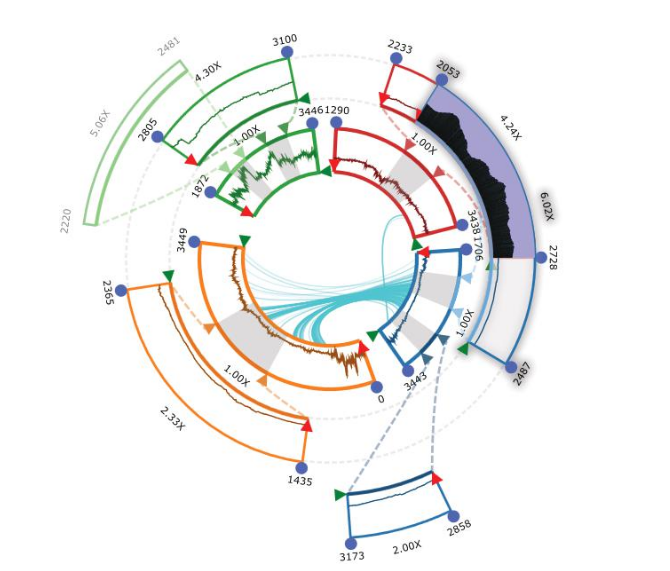
\includegraphics[width=1\textwidth]{assets/fig_7_3.png} 
    \caption{KronoMiner [488]. KronoMiner là một công cụ khám phá chuỗi thời gian đa mục đích cung cấp các tính năng điều hướng và phân tích phong phú} % Creates caption underneath graph
    \label{fig:f7.3}
\end{figure}
\subsection{Dữ liệu: Khung tham chiếu - Không gian}
Tominski và Schulz [415] giới thiệu kĩ thuật trực quan hóa cho dữ liệu thời gian có yếu tố không gian địa lý 2D và thời gian tuyến tính 1D. Ý tưởng là xây dựng một lát cắt không phẳng được gọi là \textit{Great Wall of Space-Time} (hình 7.4) thông qua không-thời gian liên tục 3D (2D+1D). Kiến trúc bức tường này được xây dựng dựa trên các khía cạnh tô tô và hình học của không gian địa lý. Dựa trên một đồ thị lân cận, một đường tô pô được thiết lập tự động hoặc có tương tác. Đường tô pô này được biến đổi thành đường địa lý thông qua những tính chất địa lý của khu vực trên bản đồ. Đường này được dựng thành một bức tường 3D mà chiều thứ 3 có thể được dùng để ánh xạ đến miền thời gian. Những biểu diễn trực quan khác nhau có thể được chiếu lên bức tường này để biểu thị dữ liệu. Bức tường có lợi thế là nó thể hiện một đường khép kín qua không gian mà không có khoảng trống giữa các pixel mang thông tin trên màn hình. 
\begin{figure}[H] % places figure environment here   
    \centering % Centers Graphic
    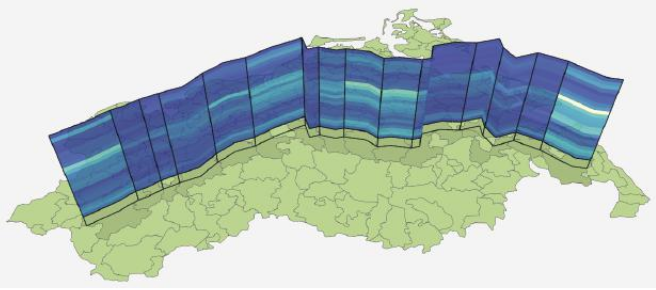
\includegraphics[width=1\textwidth]{assets/fig_7_4.png} 
    \caption{Biểu diễn trực quan hoa của dữ liệu sức khỏe con người sử dụng Great Wall of Space-Time. Một đường trong không gian được thiết lập. Dọc theo đường này, bức tường thể hiện 24 tháng của dữa lioeeuj tại mỗi vùng nó đi qua. Các màu tối thể hiện giá trị dữ liệu thấp, màu sáng thể hiện giá trị cao. Hình trên mô tả số ca mắc cúm } % Creates caption underneath graph
    \label{fig:f7.4}
\end{figure}
\subsection{Dữ liệu: Số biến - Đơn biến}
Trực quan hóa GROOVE (Granularity Overview OVErlay) [262] mở rộng trực quan hóa dựa trên pixel bằng cách phủ lên lớp tổng hợp một hoặc nhiều trong 3 phương pháp: (1) lớp phụ theo màu, (2) lớp phủ theo độ mờ hoặc (3) lớp phủ không gian. Các mức tổng hợp là kết quả của các mức độ chi tiết thời gian khác nhau. Các lớp phủ cho phép đọc vi mô và vĩ mô và trán chuyển động của mắt giữa việc quan sát tổng quan và chi tiết. Với mục đích mình họa, chúng tôi giữ sự hiển thị đơn giản và lượng dữ liệu trực quan không nhiều. Không gian trống xuất hiện do sự bất thường của việc kết hợp các chi tiết tuần và tháng. 
\\ \\
Đầu tiên, các thành phần màu có thể được sử dụng với lớp phủ màu (hình 7.5). Hình này vẽ sơ đồ dữ liệu lưu lượng trong vài tuần. 
\subsection{Dữ liệu: Số biến - Đa biến}
\textit{TimeWheel} [417] là một kỹ thuật để trực quan hóa nhiều biến phụ thuộc thời gian. TimeWheel bao gồm một trục thời gian và nhiều trục cho các biến dữ liệu khác. Trục thời gian được đặt ở trung tâm của hình vẽ để nhấn mạnh đặc tính thời gian của dữ liệu. Các trục của biến dữ liệu khác được ánh xạ bởi các màu khác nhau và dược sắp xếp theo hình tròn quanh trục thời gian. Để trực quan hóa dữ liệu, các đường tỏa ra từ trục thời gian đến mỗi trục khác thiết lập một kết nối giữa thời điểm và các giá trị dữ liệu liên quan. Những đường này tạo thành các nhịp điệu để người dùng xác định mối tương quan với trục thời gian, xu hướng hoặc ngoại lai. Mỗi mẫu như vậy có thể được phân biệt một cách rõ nhất với các trục song song với trục thời gian. Để tập trung vào trục mong muốn, người dùng có thể xoay TimeWheel. Các trục được tập trung có thể được nhấn mạnh bằng cách kéo dài ra. Các trục vuông góc với trục thời gian thì khó giải thích hơn, vì thế  chúng được làm nhạt bớt màu đi và co lại. Khám phá tương tác, bao gồm điều hướng trong thời gian được hỗ trợ thông qua các trục tương tác khác nhau.
\begin{figure}[H] % places figure environment here   
    \centering % Centers Graphic
    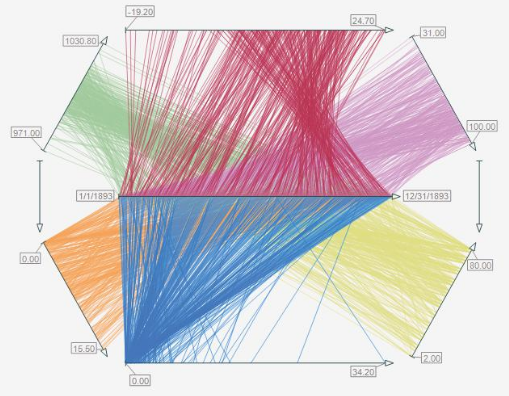
\includegraphics[width=0.8\textwidth]{assets/fig_7_7.png} 
    \caption{Trung tâm của TimeWheel [417] là trục thể hiện thời gian. Các trục khác thể hiện các biến phụ thuộc vào thời gian, hình này thể hiện 8 biến khác nhau tương ứng với 8 trục. Ở giữa, các đường đỏ thể hiện nhiệt độ trung bình, nó tăng khi bắt đầu và giảm về cuối trục thời gian. Các đường xanh dương là lượng mưa. Có một vài ngoại lại với lượng mưa cao nhưng lượng mưa cả năm thì không bất thường (Nguồn: VisAxes) } % Creates caption underneath graph
    \label{fig:f7.7}
\end{figure}
\subsection{Thời gian: Sắp xếp theo trình tự thời gian tuyến tính}
Một trong những cách đơn giản nhất để biểu diễn dữ liệu chuỗi thời gian là sử dụng hệ tọa độ Descartes với trục hoành thể hiện mốc thời gian và trục tung thể hiện giá trị biến định lượng tương ứng. Mỗi cặp gồm mốc thời gian và giá trị tương ứng được thể hiện bằng một điểm trên hệ tọa độ. Cách biểu diễn này thường được gọi là \textit{đồ thị điểm}, \textit{biểu đồ điểm}, hoặc \textit{biểu đồ phân tán} (scatterplot). Harris [170] mô tả cách biểu diễn này là một dạng đồ thị hai chiều trong đó độ lớn của các biến định lượng được thể hiện thông qua khoảng cách của mỗi điểm đến các trục tọa độ. Ngoài dạng cơ bản này còn có nhiều biến thể mở rộng khác, chẳng hạn như kỹ thuật 3D (biểu đồ lớp) hoặc kỹ thuật sử dụng nhiều ký hiệu khác nhau thay vì chỉ đơn thuần là các điểm giống nhau. Kỹ thuật này đặc biệt phù hợp trong trường hợp muốn nhấn mạnh từng giá trị riêng lẻ. Bên cạnh đó, việc biểu diễn dữ liệu bằng các thang đo chung thống nhất sẽ giúp cho người đọc có thể dễ dàng nắm bắt được thông tin một cách trực quan và chính xác nhất. 
\\ \\
Phát triển trên nền tảng của biểu đồ điểm, \textit{biểu đồ đường} cho phép ta thể hiện được mối liên hệ về mặt thời gian giữa các điểm dữ liệu thông qua việc gắn các điểm dữ liệu đó trên một đường nối. Khác với biểu đồ điểm khi tập trung nhấn mạnh vào các điểm dữ liệu riêng lẻ, rời rạc, biều đồ đường sẽ giúp ta tập trung vào xu hướng tổng quan của dữ liệu theo thời gian. Tùy thuộc vào đối tượng đang được xem xét đến ta có thể sử dụng các kiểu kết nối khác nhau giữa các điểm dữ liệu như: đường thẳng, đường bậc thang (liên tục thay đổi giá trị) hoặc đường cong Bezier. Tuy nhiên, dù sử dụng bất kỳ kiểu kết nối nào nêu trên cũng cần lưu ý rằng việc phản ánh giá trị của các điểm nằm giữa hai điểm dữ liệu đã biết đều chỉ mang tính tương đối và ta sẽ không thể đảm bảo chắc chắn về độ chính xác cho mọi điểm dữ liệu được thể hiện trên đường nối. Một vấn đề khác cần lưu ý là việc thiếu dữ liệu. Trong các trường hợp thiếu dữ liệu của một khoảng thời gian nhất định mà người phân tích bỏ qua yếu tố này và chỉ đơn thuần kết nối các điểm dữ liệu liền trước và liền sau khoảng thời gian đó thì nhiều khả năng sẽ dẫn đến những kết luận không chính xác. Do đó, cần có cách thức phù hợp để biểu diễn cho người xem ý thức được vấn đề này, chẳng hạn bằng cách sử dụng các đường nối bằng nét đứt. 
\\ \\ 
Bên cạnh các dạng biểu đồ nêu trên, ta có thể sử dụng một số dạng mở rộng và biến thể khác như: biểu đồ nhiệt, biểu đồ dải, biểu đồ đường lớp, biểu đồ miền, biểu đồ chỉ số hoặc biểu đồ kiểm soát (còn gọi là biểu đồ hành vi – quy trình) (xem [170]).   
\begin{figure}[H] % places figure environment here   
    \centering % Centers Graphic
    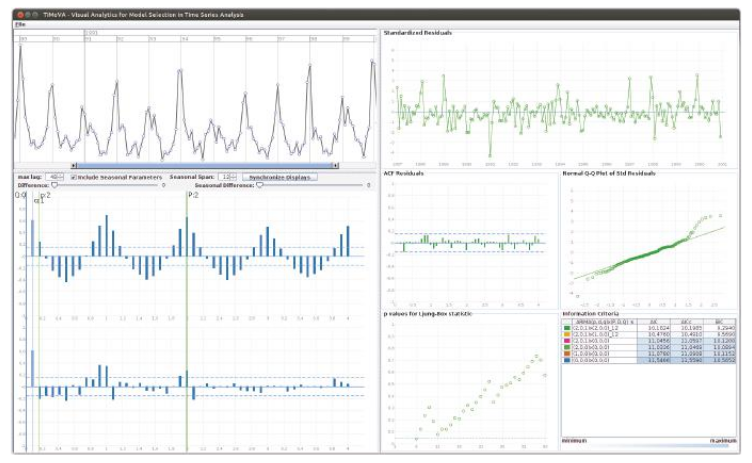
\includegraphics[width=0.8\textwidth]{assets/fig_7_8.png} 
    \caption{iMoVA. Giao diện thể hiện biểu đồ chuỗi thời gian dưới dạng biểu đồ đường (dữ liệu đầu vào; trên cùng bên trái), công cụ lựa chọn mô hình và nhiều chế độ xem khác để định hướng, hỗ trợ quá trình lựa chọn mô hình. (Nguồn: Thực hiện bằng phần mềm nguyên mẫu TiMoVA.)} % Creates caption underneath graph
    \label{fig:f7.8}
\end{figure}
Các loại biểu đồ điểm, biểu đồ đường cũng như các biểu đồ trực quan hóa khác (ví dụ: biểu đồ cột) được sử dụng một cách thường xuyên trong quá trình \textit{TiMoVA (“Ti”: Time series analysis - Phân tích chuỗi thời gian, “Mo”: Model selection - Lựa chọn mô hình, “VA”: applies Visual Analytics methods - áp dụng các phương pháp Phân tích hình ảnh trực quan)} [42]. Phân tích thống kê với dữ liệu chuỗi thời gian là một nhiệm vụ đầy thách thức và đòi hỏi phải được thực hiện bởi các chuyên gia trong nhiều lĩnh vực khác nhau, ví dụ như khi một nhân viên y tế công muốn dự đoán số người cần được điều trị tim mạch trong năm tới. Thông thường, việc lựa chọn mô hình là một nhiệm vụ phức tạp. Chính vì vậy, TiMoVA là một công cụ hữu hiệu, cung cấp giao diện tương tác để định hướng cho người dùng khai phá dữ liệu và lựa chọn mô hình chuỗi thời gian phù hợp. TiMoVA hỗ trợ chuyên gia trong các lĩnh vực ngành nghề trong việc: (1) lựa chọn thứ tự mô hình tương tác thông qua một giao diện trực quan, (2) cung cấp phản hồi về kết quả mô hình trong quá trình chọn thứ tự mô hình một cách trực quan và nhanh chóng tức thì, (3) quyết định về việc có nên cải thiện, thay đổi mô hình hay không (Hình 7.8). Một đánh giá thực nghiệm sử dụng bộ dữ liệu dịch tễ và sự tham gia đánh giá của 02 (hai) chuyên gia thống kê cho thấy TiMoVA hỗ trợ rất hiệu quả trong việc tạo ra một môi trường tương tác khám phá dữ liệu từ đó giúp lựa chọn được các mô hình phù hợp.
\subsection{Thời gian: Sắp xếp theo trình tự thời gian tuần hoàn}
Tominski và Schumann [416] sử dụng mã màu hai tông (two-tone) nâng cao của Saito và cộng sự [354] để trực quan hóa dữ liệu phụ chuỗi thời gian dọc theo hình xoắn ốc. Mỗi đơn vị khoảng thời gian được thể hiện bằng một đoạn duy nhất trên xoắn ốc. Mỗi phân đoạn được chia thành hai phần tô màu theo phương pháp tô màu hai tông. Ưu điểm của việc sử dụng phương pháp tô màu hai tông là nó giúp hiện thực hóa khái niệm tổng quan + chi tiết bằng một thiết kế trực quan. Hai màu được sử dụng trên mỗi đoạn xoắn ốc cho phép người dùng nhanh chóng nhận ra khoảng giá trị của đoạn đó (tổng quan). Nếu ta quan tâm tới một khoảng giá trị nhất định, tỷ lệ của hai màu sẽ giúp biểu thị giá trị dữ liệu cụ thể một cách chính xác (chi tiết). \textit{Xoắn ốc tương tác nâng cao} có thể được điều chỉnh tương tác theo nhiều cách khác nhau. Số lượng đơn vị giai đoạn thời gian, số chu kỳ và các tham số hình học bổ sung sẽ quyết định hình dạng của đường xoắn ốc. Việc biểu diễn dữ liệu chủ yếu được kiểm soát bởi các thang màu sắc đã sử dụng và các tham số như số lượng màu, hướng ánh xạ và chức năng ánh xạ (tuyến tính hay logarit). Việc điều hướng có thể được thực hiện tức thì thông qua việc điều chỉnh trực tiếp xoắn ốc.
\\ \\ 
Nội dung mục này và Hình (\ref{fig:f7.9}) minh họa một hình xoắn ốc nâng cao với mã màu hai tông. Mã giả dưới đây là một ví dụ minh họa cách vẽ một hình xoắn ốc đơn giản trong đó màu sắc và độ rộng của các thanh thể hiện độ lớn giá trị của dữ liệu tương ứng (so sánh hình ảnh ở giữa và bên phải trong Hình (\ref{fig:f7.1})). Các tham số đầu vào bao gồm dữ liệu (\textit{data[]}) - một mảng gồm n giá trị dữ liệu không âm với \textit{max} là giá trị lớn nhất. Tọa độ tâm của hình xoắn ốc được ký hiệu là \textit{cx} và \textit{cy}. Bán kính trong và bán kính ngoài của hình xoắn ốc được cho bởi các tham số \textit{inRad} và \textit{outRad}. Số lượng giá trị dữ liệu hiển thị trong một chu kỳ xoắn ốc đầy đủ, hay nói cách khác là số lượng đoạn thẳng trên mỗi chu kỳ được cho bởi tham số \textit{cyclLen}.
\begin{figure}[H] % places figure environment here   
    \centering % Centers Graphic
    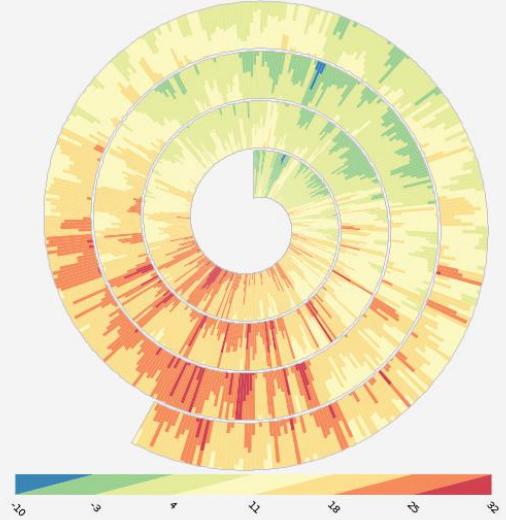
\includegraphics[width=0.8\textwidth]{assets/fig_7_9.png} 
    \caption{Xoắn ốc tương tác nâng cao [416]. Hình xoắn ốc biểu diễn dữ liệu thời tiết trong 3 năm 6 tháng. Mỗi chu kỳ thể hiện 365 giá trị nhiệt độ trung bình hàng ngày ở thành phố Rostock. Ta có thể thấy mùa đông những năm gần đây (chu kỳ ngoài cùng) có khí hậu ôn hòa hơn so với các mùa đông trước. (Nguồn: Hình vẽ được thực hiện bằng công cụ biểu diễn xoắn ốc tương tác nâng cao.)} % Creates caption underneath graph
    \label{fig:f7.9}
\end{figure}
\subsection{Thời gian: Nguyên thủy thời gian – Tức thời}
CareCruiser [163] là một hệ thống trực quan hỗ trợ việc xác định sơ bộ ảnh hưởng của các hoạt động lâm sàng đối với tình trạng của bệnh nhân. Để đạt được mục tiêu này, CareCruiser trực quan hóa các chi tiết trong pháp đồ điều trị kết hợp với các thông số của bệnh nhân, đặc biệt là thông số liên quan đến các quá trình diễn tiến thay đổi theo thời gian. Nó hỗ trợ khai phá thông tin thông qua việc căn chỉnh, đánh dấu màu, lọc và cung cấp thông tin về bối cảnh chung cũng như thông tin chi tiết cần tập trung. Sắp xếp các kế hoạch điều trị lâm sàng theo chiều dọc sẽ giúp đơn giản hóa việc so sánh hiệu quả của các phương pháp điều trị khác nhau hoặc so sánh hiệu quả khác nhau của cùng một phương pháp điều trị nhưng trên nhiều đối tượng bệnh nhân khác nhau. Bên cạnh đó, việc theo dõi hiệu quả của một hoạt động lâm sàng trong tất cả các lần thực hiện (ví dụ: sử dụng lặp lại một loại thuốc nhất định) sẽ giúp tạo điều kiện thuận lợi cho việc so sánh hiệu quả của hoạt động lâm sàng này đối với tình trạng của bệnh nhân. Ba cách phối màu khác nhau được sử dụng để làm nổi bật các phần thú vị trong quá trình phát triển một tham số: việc làm nổi bật (tô đậm) khoảng cách giữa các giá trị thực tế với giá trị dự kiến giúp xác định các giá trị quan trọng; việc làm nổi bật (tô đậm) tiến trình của các giá trị thực tế so với các giá trị ban đầu cho thấy kế hoạch điều trị được áp dụng có tác dụng như đạt mức độ nào so với mong đợi; và việc làm nổi bật độ dốc (sự thay đổi đột ngột) của một giá trị sẽ giúp ta khám phá những tác động tức thời của các hoạt động lâm sàng được áp dụng. Một thanh trượt được cung cấp để lựa chọn màu sắc làm nổi bật cho các sự kiện được chọn (xem Hình 7.10, phía trên cùng) và một cửa sổ cung cấp hình ảnh đã làm mờ thông tin màu bên ngoài đường viền được sử dụng để hỗ trợ quan sát tập trung vào một vùng cần quan tâm cụ thể (ví dụ: phần thời gian nhất định sau khi áp dụng một hành động lâm sàng). Các vùng ít được nhấn mạnh hơn một chút bên ngoài cửa sổ đã nêu trên biểu thị đường cong các giá trị liên tiếp của hoạt động, từ đó cung cấp một số thông tin ngữ cảnh xung quanh cho các giá trị nổi bật mà chúng ta đang quan tâm phân tích. 
\begin{figure}[H] % places figure environment here   
    \centering % Centers Graphic
    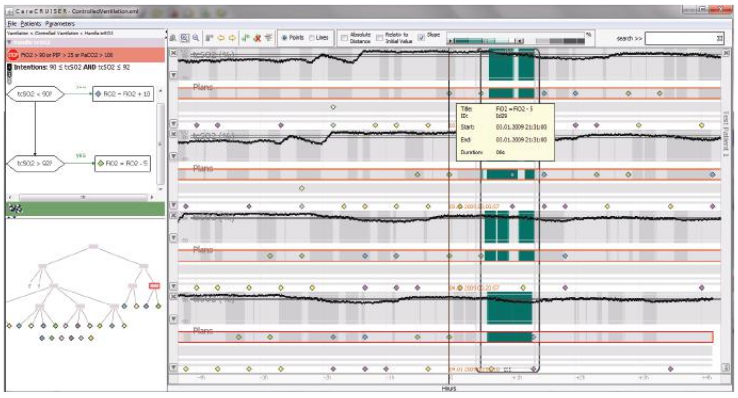
\includegraphics[width=0.8\textwidth]{assets/fig_7_10.png} 
    \caption{CareCruiser [163]. Chế độ xem theo thời gian (ở phía bên phải) sắp xếp các thông số của bệnh nhân cùng với các hoạt động lâm sàng đã được thực hiện (các chấm nhỏ bên dưới biểu đồ đường) dọc theo trục thời gian nằm ngang. Các chế độ xem theo trật tự móc nối logic và trật tự phân cấp ghi lại các kế hoạch điều trị được hiển thị ở phía bên trái. Khu vực đang được chọn ở cửa sổ bên phải thể hiện giá trị tcSO2 của bệnh nhân giảm chậm sau khi áp dụng một hoạt động lâm sàng cụ thể. (Nguồn: Thực hiện bằng phần mềm nguyên mẫu CareCruiser.)} % Creates caption underneath graph
    \label{fig:f7.10}
\end{figure}
\subsection{Thời gian: Nguyên thủy thời gian – Theo khoảng}
Đồng hồ xoắn ốc (SpiraClock) [98] trực quan hóa thời gian bằng cách sử dụng hình ảnh một chiếc đồng hồ. Hình thức thể hiện bao gồm một mặt đồng hồ và hai kim chỉ giờ và chỉ phút. Mặt trong của đồng hồ hiển thị một hình xoắn ốc kéo dài từ viền của đồng hồ về phía tâm của nó. Mỗi chu kỳ của hình xoắn ốc đại diện cho 12 giờ, với thời gian thực được hiển thị ở chu kỳ ngoài cùng và các mốc thời gian tương lai được hiển thị ở gần trung tâm (trong Hình 7.11 là khoảng 9 tiếng sau trong tương lai). Các khoảng thời gian (ví dụ: các cuộc họp) được thể hiện dưới dạng các phân đoạn được tô màu dọc theo hình xoắn ốc. Các phân đoạn này sẽ thể hiện cho ta biết được thời điểm bắt đầu và kết thúc. Từ đó, người dùng cũng có thể nhanh chóng quan sát được xem liệu các cuộc họp nhất định có bị chồng chéo nhau hay chương trình làm việc có quá dày đặc do nhiều sự kiện liên tiếp nhau hay không. Khi thời gian trôi qua, vòng xoắn ốc được cập nhật liên tục và các khoảng thời gian trong tương lai dần dần di chuyển ra ngoài cho đến khi chúng trở thành thời gian hiện tại (thời gian thực). Song song với đó, các khoảng thời gian quá khứ sẽ dần dần mờ đi. Với cách thức hoạt động như trên, SpiraClock là một phiên bản nâng cấp của chiếc đồng hồ cổ điển khi nó cho phép người dùng xem trước các khoảng thời gian của tương lai gần và đồng thời cũng có thể nắm bắt khái quát về các khoảng thời gian quá khứ. SpiraClock cũng cho phép người dùng di chuyển kim đồng hồ để truy cập tới các thời điểm khác nhau, bên cạnh đó ta cũng có thể đánh dấu để làm nổi bật các khoảng thời gian mà chúng ta quan tâm và tạo ra các ghi chú dạng văn bản kèm theo tương ứng.
\begin{figure}[H] % places figure environment here   
    \centering % Centers Graphic
    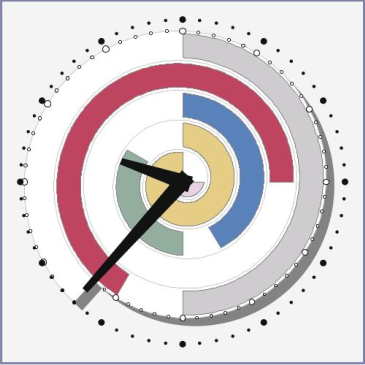
\includegraphics[width=0.8\textwidth]{assets/fig_7_11.png} 
    \caption{SpiraClock [98] được xây dựng dựa trên ý tưởng của màn hình một chiếc đồng hồ. Trong hình, kim phút hiện đang chỉ vào một cuộc họp đang diễn ra. Các cuộc hẹn trong tương lai được xếp dọc theo hình xoắn ốc trên mặt đồng hồ. (Nguồn: Tác giả tổng hợp)} % Creates caption underneath graph
    \label{fig:f7.11}
\end{figure}
\subsection{Trực quan hóa: Ánh xạ tĩnh}
PostHistory [438] khai phá trực quan các mẫu hình (pattern) hoạt động e-mail khác nhau (ví dụ: các mạng xã hội, tốc độ trao đổi e-mail) và vai trò của thời gian trong các mô hình này (xem Hình 7.12). PostHistory lấy người dùng làm trung tâm và tập trung vào các tương tác trực tiếp của một người dùng với những người khác thông qua e-mail. Các mẫu hình được tạo ra từ việc phân tích thông tin tiêu đề e-mail. Vì vậy, không phải nội dung của thư, mà lưu lượng được lưu vết mới là yếu tố được sử dụng làm cơ sở để phân tích các e-mail trao đổi của mọi người theo thời gian. Về cơ bản, giao diện người dùng trực quan hóa hoạt động trao đổi e-mail trong cả một năm và giao diện này được chia thành hai bảng chính: bảng lịch ở bên trái và bảng danh bạ ở bên phải. Bảng lịch hiển thị cường độ hoạt động e-mail hàng ngày trong đó mỗi ô vuông biểu thị một ngày và mỗi hàng biểu thị một tuần. Kích thước của hình vuông được xác định bởi số lượng e-mail nhận được vào ngày đó và màu sắc của nó thể hiện hướng trung bình tính của thư (tức là thư được nhận qua hình thức TO, CC hay BCC). Màu sắc càng sáng thể hiện các thư nhận được trong ngày hôm đó càng được định hướng rõ ràng. Bảng danh bạ được sử dụng để hiển thị tên của những người đã gửi e-mail cho người dùng.
\subsection{Trực quan hóa: Ánh xạ động}
Dữ liệu thị trường chứng khoán thay đổi linh hoạt trong ngày do giá thị trường liên tục được cập nhật trong phiên giao dịch. Vande Moere [436] đề xuất một cách thức trực quan hóa những dữ liệu như vậy bằng các chùm thông tin (\textit{flocking boids}). Thuật ngữ “boids” mượn từ sự mô phỏng của các loài chim trong đàn (các đối tượng chim = các boid). Để trực quan hóa giá thị trường chứng khoán, mỗi cổ phiếu được coi là một boid với vị trí ban đầu ngẫu nhiên trong không gian ba chiều. Khi có dữ liệu mới, các vị trí boid được cập nhật tự động theo một số quy tắc. Các quy tắc này thường được xây dựng để hướng tới các mục đích như: (i) tránh sự va chạm giữa các đối tượng di chuyển, (ii) đảm bảo tốc độ di chuyển các đối tượng trong cùng một chùm là giống nhau, (iii) các đối tượng có xu hướng di chuyển về phía trung tâm của đàn, và (iv) đảm bảo các đối tượng có độ tương đồng cao sẽ di chuyển gần nhau trong khi các đối tượng khác nhau sẽ di chuyển xa nhau. Cách thức biểu diễn trực quan hóa này có tính “động” đặc thù giúp thúc đẩy khả năng của người phân tích để nhận biết các xu hướng, mẫu hình (nếu có) khi các chùm di chuyển. Để làm được điều này, các đối tượng (boids) và đường đi của chúng phải được hiển thị dưới dạng các đường cong sinh động, như thể hiện ở Hình (\ref{fig:f7.13}) (hình bên trái). Ta cũng có thể nâng cấp cách biểu diễn trực quan 3D này bằng cách bao đóng các chùm bên trong các bề mặt ẩn, giúp người dùng có thể dễ dàng hơn trong việc nhận diện cấu trúc không gian của chùm (xem Hình (\ref{fig:f7.13}), bên phải). Các chùm có thể sẽ rất hữu ích trong việc khai phá, tìm kiếm các xu hướng, mẫu hình khác nhau trong bộ dữ liệu, chẳng hạn như sự tồn tại của các chùm dữ liệu, sự tách biệt của các chùm con khỏi chùm chính hoặc hành vi khác nhau của các đối tượng trong cùng một chùm.
\begin{figure}[H] % places figure environment here   
    \centering % Centers Graphic
    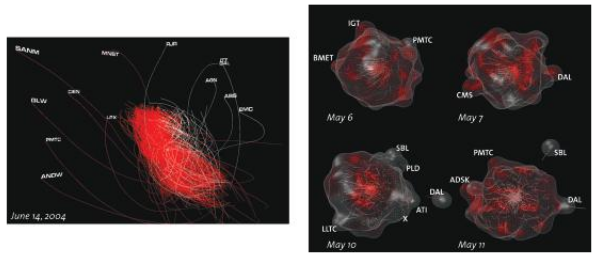
\includegraphics[width=0.8\textwidth]{assets/fig_7_13.png} 
    \caption{Chùm dữ liệu [436]. Dữ liệu thị trường chứng khoán được thể hiện dưới dạng các chùm di chuyển trong không gian ba chiều. Bên trái: các đối tượng tách khỏi chùm cho thấy giá cổ phiếu tương ứng có xu hướng vận động khác với phần lớn giá của các cố phiếu khác; bên phải: các bề mặt ẩn bao quanh các khối giúp người dùng nhận biết cấu trúc không gian của chùm.} % Creates caption underneath graph
    \label{fig:f7.13}
\end{figure}
\subsection{Trực quan hóa: Số chiều – 2 chiều (2D)}
\textit{VisuExplore} [338] là một hệ thống tương tác trực quan phục vụ cho việc khai phá chuỗi các dữ liệu, thông số y tế không đồng nhất theo thời gian. Hệ thống này sử dụng nhiều chế độ xem khác nhau nằm song song với nhau theo chiều dọc với chung một trục hoành là trục thời gian, từ đó giúp cho việc tham chiếu các thông số y tế có liên quan với nhau. VisuExplore cung cấp một môi trường mở rộng chứa các công cụ, kỹ thuật hiển thị trực quan với tôn chỉ đơn giản, dễ dàng sử dụng trong thực hành y tế như: biểu đồ đường, biểu đồ dòng thời gian (timeline), biểu đồ cột, biểu đồ miền [331], biểu đồ sự kiện, biểu đồ đường với chú thích có thể thu phóng (xem Hình (\ref{fig:f7.14}), trên cùng). Ngoài ra, dữ liệu cũng có thể được trình bày dưới dạng các bảng chứa văn bản để đa dạng các cách thức trực quan hóa. Các tính năng tương tác của VisuExplore cho phép các bác sĩ có được cái nhìn tổng quan về nhiều thông số y tế và tập trung vào các phần của dữ liệu. Có thể thêm hình ảnh hiển thị một hoặc nhiều biến bổ sung. Người dùng có thể thêm, xóa, thay đổi kích thước và sắp xếp lại các chế độ xem trực quan hóa vì VisuExplore cũng cung cấp khả năng tương tác phong phú để thêm, xóa, sắp xếp và điều chỉnh chế độ xem. Ngoài ra, một công cụ đo lường cũng được tích hợp để có thể xác định khoảng thời gian giữa các hai thời điểm mà người dùng quan tâm và lựa chọn; chức năng này không hoạt động trong phạm vi của một chế độ xem cụ thể mà còn có thể hoạt động xuyên suốt trên các chế độ xem khác nhau.
\begin{figure}[H] % places figure environment here   
    \centering % Centers Graphic
    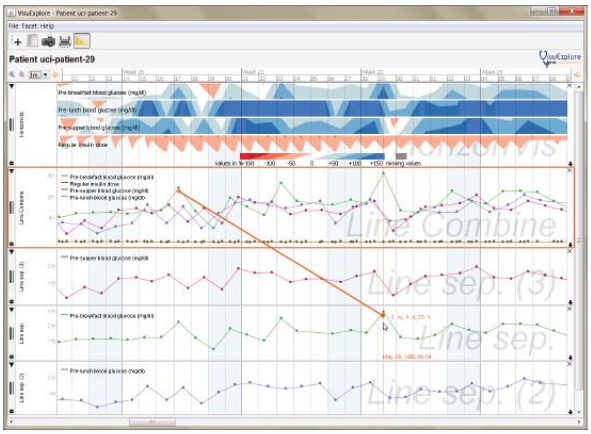
\includegraphics[width=0.8\textwidth]{assets/fig_7_14.png} 
    \caption{VisuExplore [338]. Các phương pháp biểu diễn trực quan, đơn giản và dễ hiểu bằng cách sử dụng biểu đồ đường, biểu đồ cột, biểu đồ sự kiện, biểu đồ dòng thời gian và biểu đồ đường kèm chú thích. Trong đó, công cụ đo lường được minh họa: Một đường nối minh họa cho khoảng thời gian giữa hai mục được chọn (đường nối này hoạt động trên các khung khác nhau). (Được tạo bằng phần mềm nguyên mẫu VisuExplore.)} % Creates caption underneath graph
    \label{fig:f7.14}
\end{figure}
\subsection{Trực quan hóa: Số chiều – 3 chiều (3D)}
\textit{3D ThemeRiver} [197] (xem Hình (\ref{fig:f7.15})) là một biến thể 3D của kỹ thuật ThemeRiver [172] (xem Hình 7.16). Phương pháp 3D kế thừa thiết kế hình ảnh cơ bản từ phiên bản 2D của nó: các dữ liệu chuỗi thời gian được thể hiện bằng độ rộng của các dòng có màu sắc khác nhau tạo thành một dòng chảy xuyên suốt theo trục thời gian nằm ngang. Trong biến thể 2D, chỉ có thể biểu diễn một biến dữ liệu trên mỗi dòng, cụ thể là bằng cách thay đổi độ rộng của dòng đó. Giải pháp cải tiến của Imrich et al. và các cộng sự sẽ giúp giải quyết hạn chế này. Việc mở rộng thiết kế thêm một chiều thứ ba giúp chúng ta có thể thể hiện thêm được nhiều thông tin trực quan bổ sung: chiều cao (ở dạng 3D) của mỗi dòng có thể được thay đổi để thể hiện thêm những thông tin cần thiết. Thiết kế này đặc biệt phù hợp để hình dung các xu hướng đồng biến bậc ba trong dữ liệu. Imrich và các cộng sự [197] đã tiến hành khảo sát người dùng để đánh giá tính hữu ích của việc biểu diễn 3D này và thực sự đã thu được kết quả tích cực cho thấy biến thể 3D có nhiều ưu điểm hơn so với biến thể 2D. Cụ thể, sự sẵn có của các công cụ tương tác điều hướng 3D thích hợp được nhấn mạnh là một yếu tố quan trọng góp phần vào sự thành công của 3D ThemeRiver.
\begin{figure}[H] % places figure environment here   
    \centering % Centers Graphic
    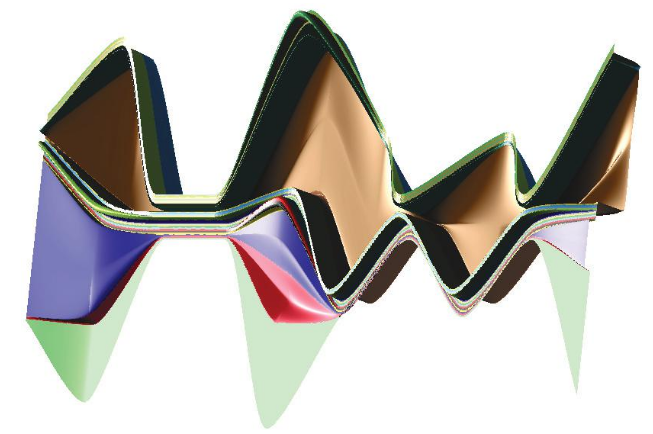
\includegraphics[width=0.8\textwidth]{assets/fig_7_15.png} 
    \caption{3D ThemeRiver [197]. Các dòng có màu riêng biệt tạo thành hình dạng tổng thể của 3D ThemeRiver. Ngoài ra, chiều rộng và chiều cao của các dòng được thay đổi để thể hiện giá trị thay đổi của dữ liệu theo thời gian. Trong hình này, chiều rộng biểu diễn sự phân bố tổng thể của 17 cụm dữ liệu aerosol và chiều cao biểu thị tỷ lệ kẽm. (Được sử dụng với sự cho phép của các tác giả.)} % Creates caption underneath graph
    \label{fig:f7.15}
\end{figure}
Bảng \ref{fig:tb7.16} cung cấp một cách tổng quan về tất cả các kỹ thuật có trong chương này cùng với  các thông tin phân loại chúng. Ta cũng có thể sử dụng bảng này để tìm kiếm các kỹ thuật trực quan hóa đáp ứng các tiêu chí nhất định.
\begin{figure}[H] % places figure environment here   
    \centering % Centers Graphic
    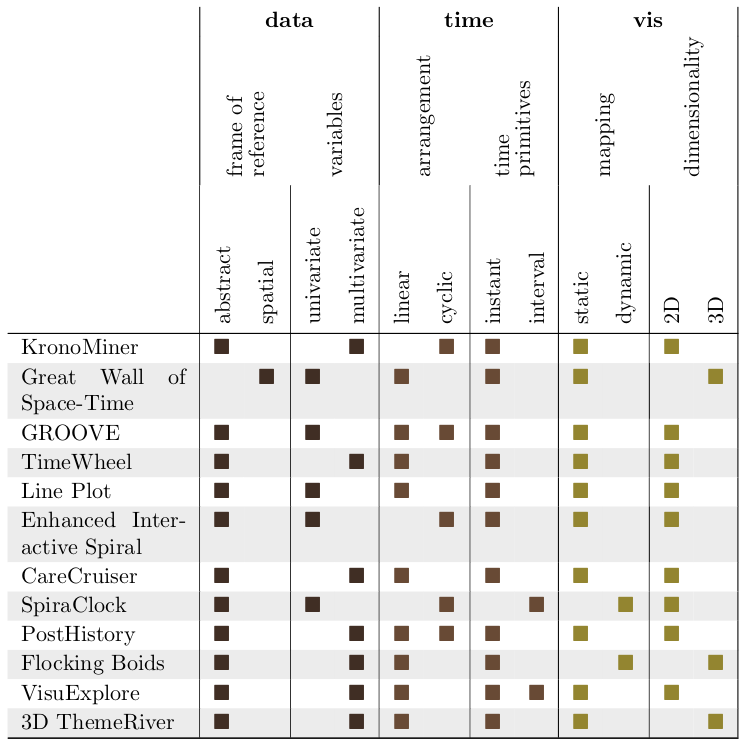
\includegraphics[width=0.9\textwidth]{assets/tb_7_1.png} 
    \caption{Tổng quan và phân loại các kỹ thuật trực quan hóa} % Creates caption underneath graph
    \label{fig:tb7.16}
\end{figure}

